%++++++++++++++++++++++++++++++++++++++++
\documentclass[article, 12pt]{article}
\usepackage{float}
\usepackage{setspace}
\usepackage{tabu} % extra features for tabular environment
\usepackage{amsmath}  % improve math presentation
\usepackage{graphicx} % takes care of graphic including machinery
\usepackage[margin=1in]{geometry} % decreases margins
\usepackage{cite} % takes care of citations
\usepackage[final]{hyperref} % adds hyper links inside the generated pdf file
\usepackage{tikz}
\usepackage{caption} 
\usepackage{fancyhdr}
\usepackage{amssymb} % symbols like /therefore
\usepackage{amsthm} % proofs
\usepackage{enumerate} % lettered lists
\usepackage{mathtools} % macros
\usepackage[all]{xy} % for diagrams
\usepackage{tkz-graph}
\usetikzlibrary{knots}
\usepackage{xcolor}
\usetikzlibrary{scopes}
% \usepackage{xcolor} \pagecolor[rgb]{0.12549019607,0.1294117647,0.13725490196} \color[rgb]{0.82352941176,0.76862745098,0.62745098039} % dark theme
\theoremstyle{definition}
\newtheorem{example}{Example}[subsubsection]
\newtheorem*{remark}{Remark}
\newtheorem{theorem}{Theorem}[subsubsection]
\newtheorem{definition}{Definition}[subsubsection]
\newtheorem{corollary}{Corollary}[subsubsection]
\hypersetup{
	colorlinks=false,      % false: boxed links; true: colored links
	linkcolor=blue,        % color of internal links
	citecolor=blue,        % color of links to bibliography
	filecolor=magenta,     % color of file links
	urlcolor=blue         
}
\usepackage{physics}
\usepackage{siunitx}
\usepackage{tikz,pgfplots}
\usepackage[outline]{contour} % glow around text
\usetikzlibrary{calc}
\usetikzlibrary{angles,quotes} % for pic
\usetikzlibrary{arrows.meta}
\tikzset{>=latex} % for LaTeX arrow head
\contourlength{1.2pt}

\colorlet{xcol}{blue!70!black}
\colorlet{vcol}{green!60!black}
\colorlet{myred}{red!70!black}
\colorlet{myblue}{blue!70!black}
\colorlet{mygreen}{green!70!black}
\colorlet{mydarkred}{myred!70!black}
\colorlet{mydarkblue}{myblue!60!black}
\colorlet{mydarkgreen}{mygreen!60!black}
\colorlet{acol}{red!50!blue!80!black!80}
\tikzstyle{CM}=[red!40!black,fill=red!80!black!80]
\tikzstyle{xline}=[xcol,thick,smooth]
\tikzstyle{mass}=[line width=0.6,red!30!black,fill=red!40!black!10,rounded corners=1,
                  top color=red!40!black!20,bottom color=red!40!black!10,shading angle=20]
\tikzstyle{faded mass}=[dashed,line width=0.1,red!30!black!40,fill=red!40!black!10,rounded corners=1,
                        top color=red!40!black!10,bottom color=red!40!black!10,shading angle=20]
\tikzstyle{rope}=[brown!70!black,very thick,line cap=round]
\def\rope#1{ \draw[black,line width=1.4] #1; \draw[rope,line width=1.1] #1; }
\tikzstyle{force}=[->,myred,very thick,line cap=round]
\tikzstyle{velocity}=[->,vcol,very thick,line cap=round]
\tikzstyle{Fproj}=[force,myred!40]
\tikzstyle{myarr}=[-{Latex[length=3,width=2]},thin]
\def\tick#1#2{\draw[thick] (#1)++(#2:0.12) --++ (#2-180:0.24)}
\DeclareMathOperator{\sn}{sn}
\DeclareMathOperator{\cn}{cn}
\DeclareMathOperator{\dn}{dn}
\def\N{80} % number of samples in plots


\usepackage{titling}
\renewcommand\maketitlehooka{\null\mbox{}\vfill}
\renewcommand\maketitlehookd{\vfill\null}
\usepackage{siunitx} % units
\usepackage{verbatim} 
\newcommand{\courseNumber}{MATH 1700}
\newcommand{\courseName}{Ideas in Mathematics}
\newcommand{\professor}{Professor Rimmer}
\newcommand{\psetName}{Portfolio Resubmission 3}
\newcommand{\dueDate}{Due: April 26, 2023}
\newcommand{\name}{Denny Cao}
\pagestyle{fancy}
\fancyhf{}% clears all header and footer fields
\fancyfoot[C]{--~\thepage~--}
\renewcommand*{\headrulewidth}{0.4pt}
\renewcommand*{\footrulewidth}{0pt}
\lhead{\name}
\chead{\courseNumber: \courseName}
\rhead{\professor}

% new theorem for questions and answers

\newtheorem{question}{Question}

\newtheorem{answer}{Answer}

\fancypagestyle{plain}{%
  \fancyhf{}% clears all header and footer fields
  \fancyfoot[C]{--~\thepage~--}%
  \renewcommand*{\headrulewidth}{0pt}%
  \renewcommand*{\footrulewidth}{0pt}%
}

% Shortcuts
\DeclarePairedDelimiter\ceil{\lceil}{\rceil} % ceil function
\DeclarePairedDelimiter\floor{\lfloor}{\rfloor} % floor function

\DeclarePairedDelimiter\paren{(}{)} % parenthesis

\newcommand{\df}{\displaystyle\frac} % displaystyle fraction
\newcommand{\qeq}{\overset{?}{=}} % questionable equality

\newcommand{\Mod}[1]{\;\mathrm{mod}\; #1} % modulo operator

\newcommand{\comp}{\circ} % composition

% Sets
\DeclarePairedDelimiter\set{\{}{\}}
\newcommand{\unite}{\cup}
\newcommand{\inter}{\cap}

\newcommand{\reals}{\mathbb{R}} % real numbers: textbook is Z^+ and 0
\newcommand{\ints}{\mathbb{Z}}
\newcommand{\nats}{\mathbb{N}}
\newcommand{\rats}{\mathbb{Q}}

\newcommand{\degree}{^\circ}

% Counting
\newcommand\perm[2][^n]{\prescript{#1\mkern-2.5mu}{}P_{#2}}
\newcommand\comb[2][^n]{\prescript{#1\mkern-0.5mu}{}C_{#2}}

% Relations
\newcommand{\rel}{\mathcal{R}} % relation

\setlength\parindent{0pt}

% Directed Graphs
\usetikzlibrary{arrows}
\tikzset{vertex/.style = {shape=circle,draw,minimum size=2em}}
\tikzset{svertex/.style = {shape=circle,draw,minimum size=.05em,font=\tiny}}
\tikzset{edge/.style = {->,> = latex'}}
\tikzset{dedge/.style = {-> = latex'}}
\tikzset{dot/.style={inner sep=1.5pt,circle,draw,fill}}

% Contradiction
\newcommand{\contradiction}{{\hbox{%
    \setbox0=\hbox{$\mkern-3mu\times\mkern-3mu$}%
    \setbox1=\hbox to0pt{\hss$\times$\hss}%
    \copy0\raisebox{0.5\wd0}{\copy1}\raisebox{-0.5\wd0}{\box1}\box0
}}}

% Sign Charts
\newdimen\tcolw \tcolw=2.5em % the column width
\edef\ecatcode{\catcode`&=\the\catcode`&\relax}\catcode`&=4
\def\sgchart#1#2{\vbox{\offinterlineskip\halign{\hfil##\quad&##\hfil\crcr\sgchartA#2,:,%
   \omit\sgchartR&\kern.2pt\sgchartS{.5\tcolw}\relax\sgchartE#1,\relax,%
   \sgchartS{.5\tcolw}\relax\cr
   \noalign{\kern2pt}&\def~{}\kern.5\tcolw\sgchartD#1,\relax,\cr}}}
\def\sgchartA#1:#2,{\cr\ifx,#1,\else $#1$&\sgchartB#2{}\expandafter\sgchartA\fi}
\def\sgchartB#1{\hbox to\tcolw{\hss$#1$\hss}\sgchartC}
\def\sgchartC#1{\ifx,#1,\else
   \strut\vrule\kern-.4pt\hbox to\tcolw{\hss$#1$\hss}\expandafter\sgchartC\fi}
\def\sgchartD#1#2,{\ifx\relax#1\else\hbox to\tcolw{\hss$#1#2$\hss}\expandafter\sgchartD\fi}
\def\sgchartE#1#2,{\ifx\relax#1\else
    \ifx~#1\sgchartS\tcolw\circ \else\sgchartS\tcolw\bullet\fi \expandafter\sgchartE\fi}
\def\sgchartR{\leaders\vrule height2.8pt depth-2.4pt\hfil}
\def\sgchartS#1#2{\hbox to#1{\kern-.2pt\sgchartR \ifx\relax#2\else
   \kern-.7pt$#2$\kern-.7pt\sgchartR\fi\kern-.2pt}}
\ecatcode
%++++++++++++++++++++++++++++++++++++++++
% title stuff

\makeatletter
\renewcommand{\maketitle}{\bgroup\setlength{\parindent}{0pt}
    \begin{flushleft}
        \textbf{\@title} \\ \vskip0.2cm
        \begingroup
            \fontsize{14pt}{12pt}\selectfont
            \courseNumber: \courseName 
            \vskip0.3cm 
            \professor
        \endgroup \vskip0.3cm
        \dueDate \hfill\rlap{}\bf{\name} \\ \vskip0.1cm
        \hrulefill
    \end{flushleft}\egroup 
}
\makeatother

\title{\Large\bf{\psetName}}
%++++++++++++++++++++++++++++++++++++++++
\begin{document}
    \maketitle
    \thispagestyle{plain}
    \section*{Worksheet 10 (Graph Theory I) Question 11}
    \textbf{John and Chrissy invite their friends Bey and Jay to dinner. Before dinner, some of them shake hands. Watching the other three people at the party, Chrissy observes that one person shakes no hands, one person shakes exactly one hand, and one person shakes exactly two hands. Nobody shakes their own hand or their partner's hand. How many hands did Chrissy shake, and how do you know?}
    \section*{Final Draft}
    \textbf{Chrissy shakes 1 hand.} 
    \begin{proof}
        Let $C$ denote Chrissy, $J_a$ denote Jay, $B$ denote Bey, and $J_o$ denote John. 
        \\[12pt]
        Let $X$ be the person who shakes no hands, $Y$ be the person who shakes one hand, and $Z$ be the person who shakes two hands.
        \\[12pt]
        As Chrissy observes that no one shakes their partner's hand, we know that $Z$ shakes both people from the other group. Since $X$ shakes no hands, it cannot be John who shakes 2 hands, as it would produce the following situation:
        \begin{figure}[H]
            \centering
            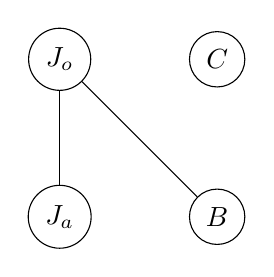
\begin{tikzpicture}
                \node[vertex] (B) at (2,-2) {$B$};
                \node[vertex] (Jo) at (0,0) {$J_o$};
                \node[vertex] (Ja) at (0,-2) {$J_a$};
                \node[vertex] (C) at (2,0) {$C$};

                \draw (Jo) -- (Ja);
                \draw (Jo) -- (B);
            \end{tikzpicture}
            \caption{John shakes 2 hands $\contradiction$} 
        \end{figure}
        The above situation depicts 4 vertices---people---with one vertex, John, with degree 2---shaking 2 hands. This situation is a contradiction, as Chrissy observed someone shaking no hands, yet there are no vertices other than Chrissy with degree 0. Therefore, $Z$ must be Jay or Bey, producing either of the following situations:
        \begin{figure}[H]
            \centering
            \begin{minipage}[t]{.4\textwidth}
                \centering
                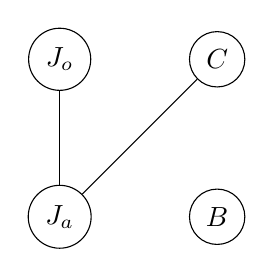
\begin{tikzpicture}
                    \node[vertex] (B) at (2,-2) {$B$};
                    \node[vertex] (Jo) at (0,0) {$J_o$};
                    \node[vertex] (Ja) at (0,-2) {$J_a$};
                    \node[vertex] (C) at (2,0) {$C$};

                    \draw (Ja) -- (Jo);
                    \draw (Ja) -- (C);
                \end{tikzpicture}
                \caption{Jay shakes 2 hands}
            \end{minipage}
            \begin{minipage}[t]{.4\textwidth}
                \centering
                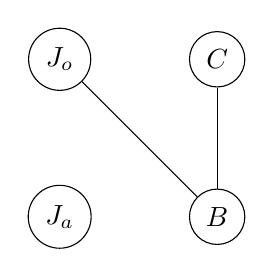
\begin{tikzpicture}
                    \node[vertex] (B) at (2,-2) {$B$};
                    \node[vertex] (Jo) at (0,0) {$J_o$};
                    \node[vertex] (Ja) at (0,-2) {$J_a$};
                    \node[vertex] (C) at (2,0) {$C$};

                    \draw (B) -- (C);
                    \draw (B) -- (Jo);
                \end{tikzpicture}
                \caption{Bey shakes 2 hands}
            \end{minipage}
        \end{figure}
        Chrissy's observations are consistent with either of these situations, as in both, there is a vertex incident to 0 edges, someone who shakes one hand, and someone who shakes two hands (or an edge with degree 0, an edge with degree 1, and an edge with degree 2):
        \begin{figure}[H]
            \centering
                \begin{tabular}{|c|c|}
                    \hline
                    Person (Vertex) & Number of Hands Shaken (Degree) \\
                    \hline
                    $J_a$ & 2 \\
                    $J_o$ & 1 \\
                    $C$ & 1 \\
                    $B$ & 0 \\
                    \hline
                \end{tabular}
                \caption{Degree of vertices when Jay shakes 2 hands}
        \end{figure}
        \begin{figure}[H]
            \centering
                \begin{tabular}{|c|c|}
                    \hline
                    Person (Vertex) & Number of Hands Shaken (Degree) \\
                    \hline
                    $B$ & 2 \\
                    $J_o$ & 1 \\
                    $C$ & 1 \\
                    $J_a$ & 0 \\
                    \hline
                \end{tabular}
                \caption{Degree of vertices when Bey shakes 2 hands}
        \end{figure}
        In both cases, Chrissy shakes one hand.
    \end{proof}
    \section*{First Draft}
    Chrissy shakes 1 hand. 
    \begin{proof}
        Let $C$ be Chrissy, $J_a$ be Jay, $B$ be Bey, and $J_o$ be John. 
        \\[12pt]
        Let $X$ be the person who shakes no hands, $Y$ be the person who shakes one hand, and $Z$ be the person who shakes two hands.
        \\[12pt]
        As Chrissy observes that no one shakes their partner's hand, we know that $Z$ shakes both people from the other group. Since $X$ shakes no hands, it cannot be John who shakes 2 hands, as it would produce the following situation:
        \begin{figure}[H]
            \centering
            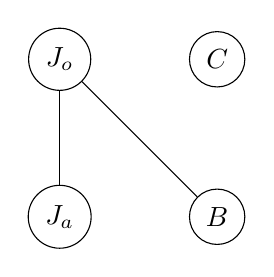
\begin{tikzpicture}
                \node[vertex] (B) at (2,-2) {$B$};
                \node[vertex] (Jo) at (0,0) {$J_o$};
                \node[vertex] (Ja) at (0,-2) {$J_a$};
                \node[vertex] (C) at (2,0) {$C$};

                \draw (Jo) -- (Ja);
                \draw (Jo) -- (B);
            \end{tikzpicture}
            \caption{John shakes 2 hands}
        \end{figure}
        This contradicts the fact that Chrissy observed someone shaking no hands. Therefore, $Z$ must be Jay or Bey, producing either of the following situations:
        \begin{figure}[H]
            \centering
            \begin{minipage}[t]{.4\textwidth}
                \centering
                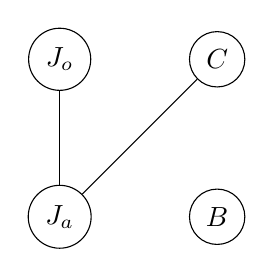
\begin{tikzpicture}
                    \node[vertex] (B) at (2,-2) {$B$};
                    \node[vertex] (Jo) at (0,0) {$J_o$};
                    \node[vertex] (Ja) at (0,-2) {$J_a$};
                    \node[vertex] (C) at (2,0) {$C$};

                    \draw (Ja) -- (Jo);
                    \draw (Ja) -- (C);
                \end{tikzpicture}
                \caption{Jay shakes 2 hands}
            \end{minipage}
            \begin{minipage}[t]{.4\textwidth}
                \centering
                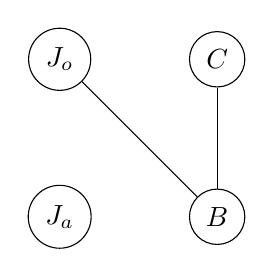
\begin{tikzpicture}
                    \node[vertex] (B) at (2,-2) {$B$};
                    \node[vertex] (Jo) at (0,0) {$J_o$};
                    \node[vertex] (Ja) at (0,-2) {$J_a$};
                    \node[vertex] (C) at (2,0) {$C$};

                    \draw (B) -- (C);
                    \draw (B) -- (Jo);
                \end{tikzpicture}
                \caption{Bey shakes 2 hands}
            \end{minipage}
        \end{figure}
        Chrissy's observations are consistent with either of these situations, as in both, there is someone who shakes no hands, someone who shakes one hand, and someone who shakes two hands. In both cases, Chrissy shakes one hand.
    \end{proof}
\end{document} 
